\documentclass{article}
\usepackage{amsmath,amssymb,amsthm}
\usepackage{enumerate}
\usepackage{mathtools}
\usepackage{graphicx}
\usepackage{caption}
\newtheorem{theorem}{Theorem}
\newtheorem{question}[theorem]{Question}
\newtheorem{answer}[theorem]{Solution}
\begin{document}
\begin{question}
	Show that the vectors $\begin{pmatrix} 
		 +2\\-1\\+1 
	\end{pmatrix}$, $\begin{pmatrix} 
	 +1\\-3\\-5 
\end{pmatrix}$ and $\begin{pmatrix} 
+3\\-4\\-4 
\end{pmatrix}$ form the vertices of a right angled triangle.
\end{question}
Solution. Let $\vec{A}$,$\vec{B}$  and $\vec{C}$ be given vectors such that $\vec{A} =\begin{pmatrix} 
	+2\\-1\\+1 
\end{pmatrix}$,\\     
$\vec{B}= \begin{pmatrix} 
+1\\-3\\-5 
\end{pmatrix}$ and $\vec{C}= \begin{pmatrix} 
+3\\-4\\-4 
\end{pmatrix}$.\\
To show that $\vec{A}$, $\vec{B}$ and $\vec{C}$ form the vertices of a right angled triangle. First we need to show that $\vec{A}$, $\vec{B}$ and $\vec{C}$ are indeed vertices of a triangle.\\
For this we need to see if the vertices satisfy triangle inequality. Let $a$, $b$ and $c$ denote the length of vectors $\vec{A}- \vec{B}$, $\vec{B}-\vec{C}$ and $\vec{C}- \vec{A}$. Now,\\
$a=\sqrt{41}$, $b=\sqrt{6}$ and $c=\sqrt{35}$. We can see that  $a+b>c$, 
$a+c>b$ and $b+c >a$. Thus, the given vectors $\vec{A}$, $\vec{B}$ and $\vec{C}$ form the vertices of a triangle.\\

\begin{figure}[!htb]
	
	\centering
	
	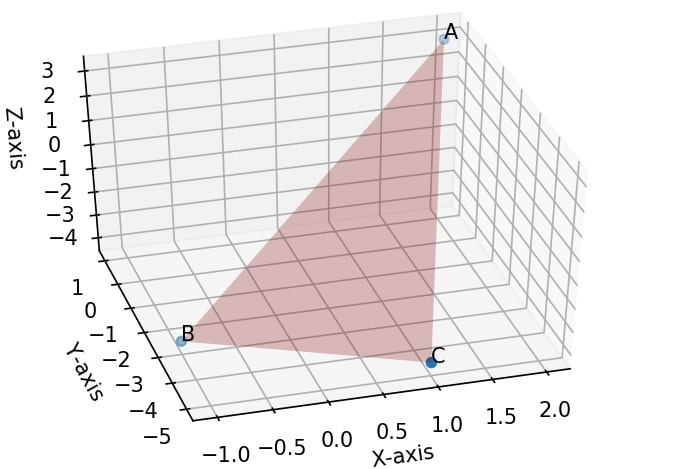
\includegraphics[width=\columnwidth]{assignment1fig-1.jpg}
	
	\caption{\label{fig1}}
	
	\label{fig:}
	
\end{figure}

To prove, the $\triangle ABC$ is a right triangle, we need to calculate the inner product of all the below vectors and check if any one of them is 0.:
\begin{enumerate}[1.]
	\item $\langle \vec{A}-\vec{C}   ,\vec{B}-\vec{C}\rangle$ = $(\vec{A} -\vec{C})^T (\vec{B}-\vec{C})$ = $(-1\;\; 3 \;\; 5)$ $\begin{pmatrix} 
		-2\\+1\\-1 
	\end{pmatrix}$ = 0
\end{enumerate}
\begin{enumerate}[2.]
	\item $\langle \vec{A}-\vec{B}   ,\vec{C}-\vec{B}\rangle$ = $(\vec{A} -\vec{B})^T (\vec{C}-\vec{B})$
	 = $(1\;\; 2 \;\; 6)$ $\begin{pmatrix} 
		+2\\-1\\+1 
	\end{pmatrix}$ = 6
\end{enumerate}

\begin{enumerate}[3.]
	\item $\langle \vec{B}-\vec{A}   ,\vec{C}-\vec{A}\rangle$ = $(\vec{B} -\vec{A})^T (\vec{C}-\vec{A})$ = $(-1\;\; -2 \;\; -6)$ $\begin{pmatrix} 
		+1\\-3\\-5 
	\end{pmatrix}$ = 35
\end{enumerate}
Clearly, from $1.$ we can see that $\triangle$ABC is right angled at C.
\end{document}
